% Sample article using the sbc20 class.
%
% The non-textual content of this file (package loading commands,
% explanatory comments, etc.) was created by Nelson Lago <lago@ime.usp.br>
% and José Viterbo Filho <viterbo@ic.uff.br>. It is licensed under the
% Creative Commons Attribution International Licence, v4.0 (CC-BY 4.0)
% https://creativecommons.org/licenses/by/4.0/
%
% Using the non-textual content of this file as a template to produce
% your own document without further attribution to the authors above
% is permitted and encouraged.
%
% charset: utf-8 ãàáâéêíõóôúç ÃÀÁÂÉÊÍÕÓÔÚÇ

% The last language is the main language of the document.
\documentclass[portuguese,notblind]{sbc20}


%%%%%%%%%%%%%%%%%%%%%%%%%%%%%%%%%%%%%%%%%%%%%%%%%%%%%%%%%%%%%%%%%%%%%%%%%%%%%%%%
%%%%%%%%%%%%%%%%%%%%%%%%%%%%%%%%%% PACKAGES %%%%%%%%%%%%%%%%%%%%%%%%%%%%%%%%%%%%
%%%%%%%%%%%%%%%%%%%%%%%%%%%%%%%%%%%%%%%%%%%%%%%%%%%%%%%%%%%%%%%%%%%%%%%%%%%%%%%%

% Basics
\usepackage{verbatim}  % support for unformatted text, almost mandatory
\usepackage{graphicx}  % support for figures etc., almost mandatory
\usepackage{array}     % extra table features, almost mandatory
\usepackage{pbalance}  % equal heights in last page columns (demands additional LaTeX passes)
\usepackage{mathtools} % extra visual tweaks/features for math, read the docs

% Table improvements
\usepackage{booktabs}  % better table aesthetics, recommended, read the docs
\usepackage{multirow}  % table cells that span over multiple rows
\usepackage{makecell}  % better table headings / cells with linebreaks inside
\usepackage{dcolumn}   % align numeric columns on the decimal separator (siunitx also offers this)
\usepackage{longtable} % multi-page tables
\usepackage{threeparttable} % tables with "footnotes"
%\usepackage{colortbl}  % colored table cells
%\usepackage{csvsimple} % load a csv file and format as table

% Extra features for floats
\usepackage{rotating}   % \sidewaystable, \sidewaysfigure, and other rotation commands
\usepackage[above,below]{placeins} % manually control float placement, read the docs
\usepackage{subcaption} % subfigures (side by side) with subcaptions (pkg subfigure is deprecated)
\usepackage{adjustbox}  % resize, clip etc. for any material, not only floats

% Source code syntax highlighting
%\usepackage{listings} % good and simple
%\usepackage{minted}   % excellent, but depends on pygments (python, free software)

%\usepackage{siunitx} % Numbers: units, scientific notation, better presentation for large numbers

%\usepackage{pdfcomment} % useful in the writing/reviewing phase


%%%%%%%%%%%%%%%%%%%%%%%%%%%%%%%%%%%%%%%%%%%%%%%%%%%%%%%%%%%%%%%%%%%%%%%%%%%%%%%%
%%%%%%%%%%%%%%%%%%%%%%%%%%%%%%% ARTICLE METADATA %%%%%%%%%%%%%%%%%%%%%%%%%%%%%%%
%%%%%%%%%%%%%%%%%%%%%%%%%%%%%%%%%%%%%%%%%%%%%%%%%%%%%%%%%%%%%%%%%%%%%%%%%%%%%%%%

% With bibLaTeX, the bibliographic databases are defined in the preamble.
% Call \addbibresource multiple times to use more than one file.
\addbibresource{bibliografia.bib}

\metadata
  {
    pubname={Simpósio Brasileiro de Alguma Área de Pesquisa},
    pubacron={SBAAP},
    idjems={XXX},
    copyrightyear=2025,
    category={Artigo Completo/Full Paper},
    bibstyle=sbc20,
    %bibstyle=sbc20-authordate,
    %nocolorlinks, % disable colored hyperlinks, for B&W printing
  }
  
\title
  {
    mainlanguagetitle={Exemplo de uso do template da SBC para artigo a ser publicado em anais de eventos na SOL em português},

    translatedtitle={Example of use of the SBC template for papers written in Portuguese to be published in SOL event proceedings},
  }

% These are used in the headers and are optional; if not
% defined, the complete title and all authors will appear
\shortauthor{Viterbo et al. 2025}
\shorttitle{Exemplo de artigo em Português para a SOL}
  
\author
  {
    % special chars in email addresses (%, _, $, &, #, ~ etc.)
    % are ok if the whole address is within braces
    email=viterbo@ic.uff.br,
    % orcid code must be written without "http://orcid.org/"
    orcid=0000-0002-0339-6624, 
    institutionID=UFF,
    country=BR,
    firstName=José,
    lastName=Viterbo 
  }
  

\author
  {
    email=lago@ime.usp.br,
    orcid=0000-0002-4306-8078,
    % institutionID may be called multiple times or include multiple items separated by commas (within braces)
    institutionID={USP,UPa},
    % institutionID={usp,upa},
    country=BR,
    firstName=Nelson~Silva,
    lastName=Lago
  }
  

  \author
  {
    email=rmvieira@inf.ufrgs.br,
    orcid=0009-0009-1113-0867,
    institutionID={UFRGS},
    country=BR,
    firstName=Raphael~Malinski,
    lastName=Vieira
  }


\author
  {
    email=granville@inf.ufrgs.br,
    orcid=0000-0001-8956-8660,
    institutionID=UFRGS,
    country=BR,
    firstName=Lisandro,
    lastName=Granville
  }


%For your affiliation, in the institution field, provide only the name of your top-level academic/research organization. This information the only relevant information for most citation databases. Use the "extraAffiliationsLast" field to include additional details about your affiliations, such as position or department.

%If possible, to ensure standardization and correct accounting of this publication for your institution, please use your institution's name in one of the forms presented in the Research Organizations Register (ROR):

%https://ror.org/

%ROR ID https://ror.org/02rjhbb08
\institution{UFF}{Universidade Federal Fluminense}

%ROR ID https://ror.org/036rp1748
\institution{USP}{Universidade de São Paulo}

\institution{UPa}{Universidade de Pasárgada}

%ROR ID https://ror.org/041yk2d64
\institution{UFRGS}{Universidade Federal do Rio Grande do Sul}

% As discussed before, if necessary, this space can be used to detail/complement information about authors and their affiliations. This item is optional...
\extraAffiliationsLast{José Viterbo é Prof. Associado do Instituto de Computação da UFF e Diretor de Publicações da SBC. Nelson Lago é pesquisador do Centro de Competência em Software Livre da USP e da Escola de Artes, Ciências e Humanidades da UPa. Raphael Malinski Vieira é aluno do curso de Bacharelado em Ciência da Computação da UFRGS. Lisandro Granville é Prof. Titular do Instituto de Informática da UFRGS e Diretor Financeiro da SBC.}

\abstract
  {
    This text, in scientific article format, aims to demonstrate the use of the new SBC template for papers to be published at SOL event proceedings, describing its main characteristics and explaining how it should be used for papers written in Portuguese. We suggest that the summary in Portuguese be between 500 and 750 words, but the organizers of each event can establish other limits.
  }

\resumo
  {
    Este texto, em formato de artigo científico, tem por objetivo demonstrar o uso do novo template para artigos da SBC para anais de eventos da SOL, descrevendo suas principais características e explicando como deve ser utilizado para artigos em português. Sugerimos que o resumo em português tenha entre 500 e 750 palavras, mas os organizadores de cada evento podem estebelecer outros limites.
  }

\keywords{Proceedings \sep Template \sep SBC OpenLib \sep Indexing}

\palavraschave{Anais de evento \sep Modelo \sep SBC OpenLib \sep Indexação}

% These are all optional; they appear at the end of the document

\contributeinfo{JV elaborou a primeira versão do template e os textos explicativos. NSL aprimorou o modelo. LG propôs a inclusão de metadados no PDF gerado e RMV implementou esta proposta.}

\acknowledgements{Agradecimentos a colegas, colaboradores etc. Essa declaração é opcional, se não houver nenhum agradecimento, pode ser deixada em branco}

\funding{Indicação de agências financiadoras etc. Essa declaração é opcional, se não houver nenhum financiamento, pode ser deixada em branco.}

\datainfo{
  Links para dados  e materiais adicionais disponíveis, como código, página do projeto etc. Essa declaração é obrigatória. Se os dados não forem disponibilizados previamente, pode-se declarar: ``Os dados e/ou materiais adicionais poderão ser disponibilizados mediante solicitação''.
}

\furtherinfo{Informações adicionais relevantes, como, por exemplo, a aprovação em comitê de ética ou o uso de ferramentas de IA generativa no desenvolvimento do artigo. Essa declaração é opcional, se não houver nada a ser acrescentado, pode ser deixada em branco}

\SBCprintbibliography
%%%%%%%%%%%%%%%%%%%%%%%%%%%%%%%%%%%%%%%%%%%%%%%%%%%%%%%%%%%%%%%%%%%%%%%%%%%%%%%%
%%%%%%%%%%%%%%%%%%%%%%%%%%%%%%%%% BEGIN TEXT %%%%%%%%%%%%%%%%%%%%%%%%%%%%%%%%%%%
%%%%%%%%%%%%%%%%%%%%%%%%%%%%%%%%%%%%%%%%%%%%%%%%%%%%%%%%%%%%%%%%%%%%%%%%%%%%%%%%

\begin{document}

\maketitle

\section{Introdução}
\label{sec:intro}

A SBC OpenLib\footnote{\url{sol.sbc.org.br}} é a nova biblioteca digital da Sociedade Brasileira de Computação (SBC), e tem como objetivo principal viabilizar o acesso à informação especializada em Computação. Seu acervo é composto por anais de eventos, periódicos de visibilidade nacional e internacional, livros e capítulos resultantes da produção científica efetuada no âmbito da SBC, oferecendo acesso aberto a todas as publicações.

Este texto, em formato de artigo científico, tem por objetivo apresentar o novo modelo para artigos da SBC, descrevendo suas principais características, explicando como deve ser utilizado e apresentando exemplos práticos. Esta versão, mais especificamente, deve ser utilizada como referência exclusivamente para a elaboração de artigos escritos em português que serão publicados em alguma série de anais de eventos na SBC OpenLib.

Este mesmo modelo deve ser adotado tanto para artigos completos quanto artigos curtos, cabendo aos organizadores de eventos definirem os limites máximos e mínimos para o número de páginas em cada caso. A Tabela~\ref{tab:equivalence} mostra a correspondência do número de páginas entre o novo modelo e o antigo modelo de artigos da SBC, a fim de orientar os organizadores de eventos na transição de modelos. 

% TODO: Mudamos o tamanho da fonte, é preciso recalcular isto! -> fiz um experimento com blind text, a proporção foi 9:6, ou seja, esta tabela parece ok.
\begin{table}[!hb]
\centering
\begin{tabular}{@{}cc@{}}
\toprule
Template antigo & Template 2025 \\
\midrule
 4  & 3 \\
 6  & 4 \\
 8  & 6 \\
 12  & 8 \\
\bottomrule
\end{tabular}
\caption{Correspondência do número de páginas considerando o modelo de artigos da SBC antigo e o novo modelo lançado em 2025.\label{tab:equivalence}}
\end{table}

A Figura~\ref{fig:page-layout} apresenta o \emph{layout} de página. As próximas seções apresentam informações detalhadas sobre cada parte do modelo. Na Seção 2, descrevemos os detalhes do cabeçalho do artigo. Na Seção 3, descrevemos os detalhes da abertura do artigo. Na Seção 4, descrevemos as seções e subseções do documento. Na Seção 5, descrevemos o uso de tabelas, figuras e algoritmos no artigo. Na Seção 6, discutimos as formas de citações e a inclusão de referências.

% TODO: if there will not be a footer, remove it from the figure
\begin{figure}
  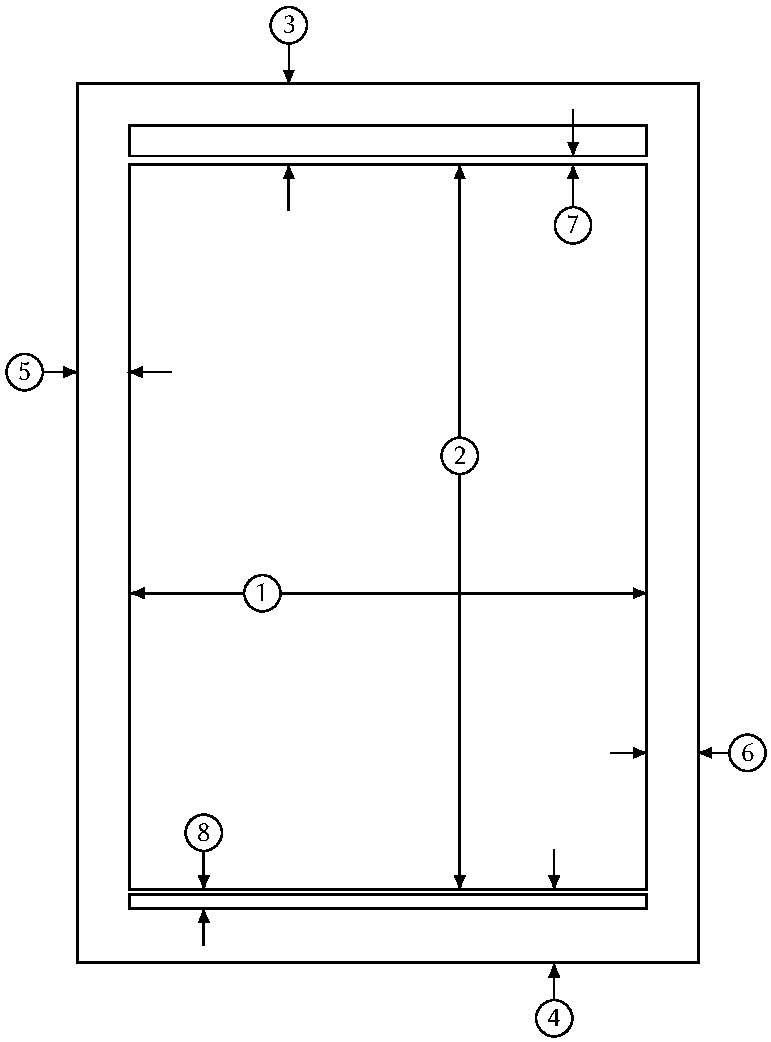
\includegraphics[width=\columnwidth]{figures/page-layout}
  \caption{\emph{Layout} da página. O tamanho é A4 (210\,x\,297\,mm);
  a mancha de texto (1 e 2) mede 175\,x\,246\,mm; a margem superior
  (3) é 26\,mm e a margem inferior (4) é 23\,mm; as margens esquerda
  (5) e direita (6) medem 17,5\,mm; o espaço entre o cabeçalho e o
  texto (7) é 10\,pt; a distância entre o final do texto e o final do
  rodapé (8) é 18\,pt; o espaço entre as colunas (não mostrado) é
  18\,pt.\label{fig:page-layout}}
\end{figure}

\section{Cabeçalho}

O cabeçalho do artigo tem duas variações, uma para a primeira página e outra para as páginas seguintes. Ambas são descritas nas subseções a seguir.

\subsection{Cabeçalho da Primeira Página}

Na primeira página, o cabeçalho apresenta o título da série e o ano da edição em uma primeira linha. A segunda linha traz a descrição da licença de publicação, que para os eventos que disponibilizam seus artigos na SBC OpenLib corresponde à licença CC BY 4.0. Os autores devem preencher a informação do título da série, acrônimo do evento e ano do evento nos campos \textit{jtitle}, \textit{jid} e \textit{jyear}, respectivamente. A informação sobre a licença deve constar do campo \textit{copyrightstatement}.

\subsection{Cabeçalho da Página 2 em diante}

A partir da página 2, o cabeçalho apresenta o título resumido à esquerda e a lista de autores resumida à direita. O título abreviado do artigo e a lista abreviada de autores devem ser preenchidos em \textit{shorttitle} e \textit{shortauthors}, respectivamente.

\section{Abertura}

O preâmbulo do artigo contém os principais metadados que descrevem o artigo: o título, o resumo e as palavras-chave, tanto em inglês, quanto em português.

\subsection{Título}

\subsection{Autores}

\section{Bibliografia}

Citações e referências bibliográficas devem seguir o formato definido pela ABNT (NBR\,10520, versão 2002 e NBR\,6023 versão 2002 ou, preferencialmente, 2018). Os organizadores de cada evento definem se as citações seguirão o formato numérico ou autor-data. Observe que:

\begin{itemize}
  \item Endereços web (URLs) não são colocados entre ``<\,>'' (esse é o padrão na versão 2018 da NBR\,6023)
  \item ``In'' e ``et al.'' são formatados em itálico (esse é o padrão na versão 2018 da NBR\,6023)
  \item No formato numérico, os sobrenomes não são grafados em caixa alta
  \item No formato autor-data, usa-se versalete para os sobrenomes (com a primeira letra maiúscula)
\end{itemize}

\section{Outros exemplos}

Esta classe é baseada na classe \texttt{article} e, portanto, os comandos usuais de \LaTeX, como \textsf{\textbackslash{}verse}, \textsf{\textbackslash{}quotation} etc. podem ser usados normalmente:

\begin{verse}
Batatinha quando nasce\\
Espalha a rama pelo chão

A menina quando dorme\\
Põe a mão no coração
\end{verse}

\begin{quotation}
\itshape
Algum tempo hesitei se devia abrir estas memórias pelo princípio ou
pelo fim, isto é, se poria em primeiro lugar o meu nascimento ou a
minha morte. Suposto o uso vulgar seja começar pelo nascimento,
duas considerações me levaram a adotar diferente método: a
primeira é que eu não sou propriamente um autor defunto, mas um
defunto autor, para quem a campa foi outro berço; a segunda é que
o escrito ficaria assim mais galante e mais novo. Moisés, que também
contou a sua morte, não a pôs no intróito, mas no cabo: diferença
radical entre este livro e o Pentateuco.
\end{quotation}

Equações de segundo grau (Equação \ref{eq:2grau}) são estudadas no ensino
médio. As raízes de uma equação de segundo grau podem ser encontradas
por~\eqref{eq:bhaskara} --- a fórmula de Bháskara. O valor do discriminante
$\Delta$ (Equação \ref{eq:delta}) determina se a equação tem zero, uma ou
duas raízes reais distintas.

\begin{equation}
  \label{eq:2grau}
  ax^2+bx+c=y \quad \forall x \in \mathbb{R}
\end{equation}

\begin{gather}
  \label{eq:bhaskara}
    y=0 \Leftrightarrow x=\frac{-b \pm \sqrt{\Delta}}{2a}
    \Leftrightarrow x \text{ é raiz da equação}\\
  \label{eq:delta}
    \Delta\enspace(\mathit{delta}) = b^2-4ac
\end{gather}

\begin{figure}
  \centering
  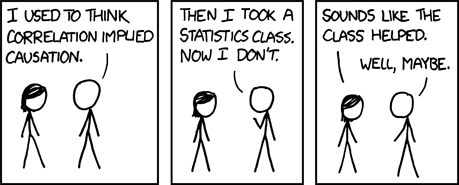
\includegraphics[width=\columnwidth]{figures/xkcd_552_correlation}
   \caption{A bitmap figure (from \url{xkcd.com/552}).\label{fig:xkcd-correlation}}
\end{figure}

\begin{figure*}[b]
  \centering
  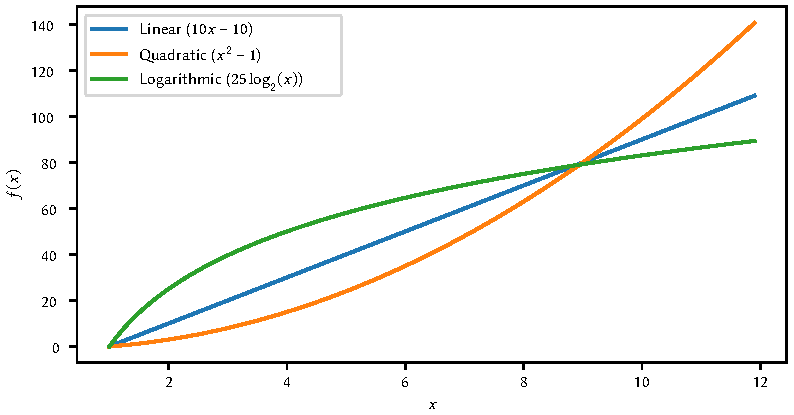
\includegraphics{figures/graph-functions}
  \caption{A vector figure spanning both text columns.\label{fig:graph-functions}}
\end{figure*}

Imagens vetoriais (como diagramas e gráficos, a exemplo das Figuras~\ref{fig:page-layout}~e~\ref{fig:graph-functions}) \emph{não} devem ser convertidas para \emph{bitmaps}, mas sim mantidas em algum formato vetorial, como PDF. Imagens não-vetoriais com cores predominantemente sólidas (como a Figura~\ref{fig:xkcd-correlation}) devem ser convertidas para o formato PNG e imagens fotográficas ou com texturas devem ser convertidas para o formato JPEG. Uma figura ou tabela muito grande (Figura~\ref{fig:graph-functions}, Tabela~\ref{tab:form}) pode excepcionalmente ocupar a largura das duas colunas de texto, mas apenas no início ou no final da página. Todas as figuras e tabelas devem ser acompanhadas das respectivas legendas explicativas numeradas logo abaixo delas.

\begin{table*}
  \centering
  \newcolumntype{M}[1]{>{\centering}m{#1\textwidth}}
  \begin{threeparttable}
    \begin{tabular}{|M{0.265}|M{0.073}|M{0.084}|M{0.073}|M{0.073}|M{0.08}|M{0.082}|M{0.067}|}
        \hline
      \textbf{Experimento número:} & \multicolumn{2}{c|}{1} & \multicolumn{4}{c|}{\textbf{Data:}} & jan 2017
        \tabularnewline \hline
      \textbf{Título:} & \multicolumn{7}{c|}{Medições iniciais}
        \tabularnewline \hline
      \textbf{Tipo:} & \multicolumn{7}{c|}{Levantamento quantitativo}
        \tabularnewline \hline \hline
      \textbf{Locais}          & São Paulo & Rio de Janeiro & Porto Alegre & Recife & Manaus & Brasília & Rio Branco
        \tabularnewline \hline
      \textbf{Valores obtidos} & 0.2       & 0.3            & 0.2          & 0.7    & 0.5    & 0.1      & 0.4\tnote{a}
        \tabularnewline \hline
    \end{tabular}
    \begin{tablenotes}
      \item[a] This is an example of table footnote with a reference
      \item This is an example of table footnote without a reference
    \end{tablenotes}
    \caption{A table spanning both text columns.\label{tab:form}}
  \end{threeparttable}
\end{table*}

\section{Conclusion}

\begin{itemize}
  \item @Book: \cite{Knuth:96}.

  \item @Article (em periódico): \cite{floats2014}.

  \item @InProceedings (ou @Conference): \cite{alves03:simi}.

  \item @InCollection (capítulo de livro ou coletânea): \cite{bobaoglu93:concepts}.

  \item @PhdThesis: \cite{garcia01:PhD}.

  \item @MastersThesis: \cite{schmidt03:MSc}.

  \item @Techreport: \cite{alvisi99:analysisCIC}.

  \item @Manual: \cite{biblatex}.

  \item @Misc: \cite{gridftp}.

  \item @Online (para referência a artigo \emph{online}): \cite{fowler04:designDead}.

  \item @Online (para referência a página web): \cite{FSF:GNU-GPL}.

  \item @article (para referência a página web): \cite{alon09:how}.
  
\end{itemize}


%%%%%%%%%%%%%%%%%%%%%%%%%%%%%%%%%%%%%%%%%%%%%%%%%%%%%%%%%%%%%%%%%%%%%%%%%%%%%%%%
%%%%%%%%%%%%%%%%%%%%%%%%%%%%%%%%% BIBLIOGRAPHY %%%%%%%%%%%%%%%%%%%%%%%%%%%%%%%%%
%%%%%%%%%%%%%%%%%%%%%%%%%%%%%%%%%%%%%%%%%%%%%%%%%%%%%%%%%%%%%%%%%%%%%%%%%%%%%%%%

\end{document}
